% !TEX root = ./report.tex

\clearpage
\section{The Inliner}
\label{scheme:start}

\todo[inline]{Introduce section with how the RVSDG helps with the different
steps in the below enumerated list.}

The inliner of this project performs the following when given an RVSDG as input:

\begin{enumerate}
	\item For all recursive environments ($\phi$-regions):

	\begin{enumerate}
		\item Use the approach described in
Section~\ref{sub:scheme:inlining_recur_apply_nodes} to fill a list of
\textit{loop breakers}. These $\lambda$-nodes are \textit{not} to be inlined.
		\label{MakeLoopBreakerListItem}
	\end{enumerate}

	\item Scan through the RVSDG, finding all \applyNode s. Exclude all function
calls to loop breakers, calls invoking functions that are not-statically known,
or external functions.
	\label{ScanForApplyNodesItem}

	\item Make a list of the \applyNode s found in
Step~\ref{ScanForApplyNodesItem}, and order the list of according to the
heuristics discussed in Section~\ref{sub:scheme:ordering_apply_nodes}.
The order of \applyNode s inlined can affect the amount of \applyNode s inlined,
even when each \applyNode~is evaluated with the same heuristic.
	\label{OrderApplyNodesFoundItem}

	\item Look at each \applyNode~in turn from the list made in
Step~\ref{OrderApplyNodesFoundItem} and decide whether or not to inline it
according to the heuristic discussed in \ref{sub:scheme:inlining_apply_nodes}:
	\label{LookAtNextCallSiteItem}

	\begin{enumerate}
		\item If the \applyNode~is inlined, add any newly copied (inlined)
\applyNode s, following the same criteria as used in
Step~\ref{ScanForApplyNodesItem}, to the list of \applyNode s. Continue with
Step~\ref{OrderApplyNodesFoundItem}.

		\item If the \applyNode~is not inlined, continue with
Step~\ref{LookAtNextCallSiteItem}, evaluating the next \applyNode .
		\label{InlineCallSiteItem}
	\end{enumerate}

	\item When the inliner reaches the end of the list, no more \applyNode s
have been inlined, and the inliner is finished.
\end{enumerate}

\subsection{Deciding which recursive functions to inline}
\label{sub:scheme:inlining_recur_apply_nodes}

The inliner evaluates all functions, recursive or not, with the same heuristic,
described in Section~\ref{sub:scheme:inlining_apply_nodes}. However, the inliner
of this project only evaluates \textit{some} of the \applyNode s invoking
recursive functions, to ensure termination of the compiler.

A $\phi$-region will always contain a Strongly Connected Component call
dependency graph or the recursive functions inside represented by
$\lambda$-nodes. Hence, if there's only one function present inside of a
$\phi$-region, it's always marked as a \textit{loop breaker}.

Hence, the inliner has a list of recursive functions which it knows \textit{not}
to inline, to ensure termination of the compilation. All other remaining
recursive functions may then be safely inlined with the same criteria as any
non-recursive functions.

\subsection{The order of call sites inlined}
\label{sub:scheme:ordering_apply_nodes}

\todo[inline]{Need reference to further ideas related to ordering of inlining.}

The inlining conditions we use as criteria for whether or not to inline, only
look at the properties of the function a call site invokes. Hence, when a
successive series of functions call one another, we only consider one at a time.
Thus, the ordering of the \applyNode s we look at when deciding whether or not
to inline them, matters because inlining opportunities might be missed with one
ordering, and unveiled with another.

Figure~\ref{fig:inline_ordering_ex} illustrates the different outcomes dependent
upon the order we visit each call-site (\applyNode ). If our criteria for
inlining is that the inlined function does not exceed the inlining condition: SC
$> 4$, we can inline $\lambda_1 \Rightarrow \lambda_2 \Rightarrow \lambda_3$.
However, if we inline the functions in the opposite order, $\lambda_3
\Rightarrow \lambda_2$, then the combined function $\lambda_{2+3}$ will have a
SC exceeding the given limit.

\begin{figure}[H]
	\centering
	\includegraphics[width=0.75\textwidth]{figures/inline_ordering_ex}
	\caption{A minimal example of an RVSDG subgraph, depicting a function call
order in a program.}
	\label{fig:inline_ordering_ex}
\end{figure}

\subsection{Inlining a call site}
\label{sub:scheme:inlining_apply_nodes}

To effectively test for an apt heuristic when deciding whether or not to inline
a call site, our approach is based on previous
work~\cite{deshpande2012statically}\cite{AdaptvCompilAndInlingWaterman}. This
approach utilizes something we call \textit{Inliner Conditions} (ICs) which
evaluate the function invoked by the call site. An IC evaluates a specific
property of the function invoked by \applyNode .

The inliner used several different ICs, \textit{Statement Count} (SC) and
\textit{Static Call Count} (SCC) being among these. Using ICs in this way allows
us to write and re-write inlining heuristics effectively, since we can write
them using CNF in the following fashion:
\lstinline"SC < X || SCC < Y || (SCC < Z && LND > W)"

Utilizing the inlining conditions described in
Section~\ref{sub:meth:inlining_conditions}, heuristics evaluating the function
invoked by each \applyNode~can be written in \textit{Conjunctive Normal Form}
(CNF). This enables an efficient way to search the parameter space for optimal
parameters for the inlining heuristics.

The inliner evaluates each \applyNode~with the given heuristic, and decides
whether or not to inline the call site this \applyNode~represents, depending on
the properties of the function it invokes.

\todo[inline]{Describe the algorithm and inliner conditions we land for
evaluating a call site on after testing.}
